\section{Introduction}
\label{sec:intro}

Here are some important things we need to make in the paper:
\begin{itemize}
  \item Showing why we need schema (skeleton + constraint) as 
        the representation. We need to eyeball relations in PATTY
		and make sure at least 5\% relations need a complex structure
		instead of a single path.
  \item Does our schema based method outperforms state-of-the-art and
        simple skeleton-based method? We need to construct a biased
		dataset (made up of complex relations) then test on both KBC
		and QA dataset, showing the result.
  \item Does our method work well in a regular (without bias) data?
        The current KBC result gives us the confidence, but maybe
		we need to have a try on QA dataset?
  \item The depth of our method. (Which is the weakest part, therefore
        our result must be good.)
\end{itemize}

Here are the main contributions of our paraphrasing work:
\begin{itemize}
  \item Our work generalizes skeleton representation into schema, 
        which enlarges the expressiveness for long-tail and complex
		relations.
  \item We propose an efficiency searching strategy to generate
        schema candidates with high quality.
  \item We propose a data-driven method, which learns to pick the 
        most suitable schemas from a big candidate set.
  \item Our results on KBC, QA outperforms state-of-the-art.
  \item We show a preliminary result on relation similarity task
        based on learned schema lists.
\end{itemize}

Other things to keep in mind:
\begin{itemize}
  \item Shall we stop using ``schema'', but change another name?
  \item Why we can't make a full generation at schema level? 
        (Complexity and overfix, explain it theoretically)
  \item Solve sparse matrix format in Theano's training code.
\end{itemize}


%\begin{itemize}
%\item Binary predicates in standard knowledge base are identified by certain 
%canonical forms (e.g., parent\_of), sometimes even crytic (e.g., ...)
%To support natural language queries (in QA e.g.), we need to map natural
%language predicates to predicates (or a set of connected predicates, which
%we call schema) in the knowledge base. 
%(e.g., the mother of $\rightarrow$ parent\_of and 
%gender = female. Maybe a figure here). We need to argue why this problem
%is critical and a must in QA (and other important applications).
%\item State of the arts in solving this problem (give some cites and brief
%descriptions) and their limitations. Say informally what are the challenges 
%in this problem.
%\item Our approach is to define graph schema inferred
%from the knowledge graph. We formalize the problem as given a set of
%entity pairs extracted by a natural language predicate, return a set of graph
%schemas that cover all the entities pairs and simultaneously optimizes 
%a the cost of transmitting the pairs and the schemas, according to the
%minimal description length (MDL) principle. The optimization problem is shown
%to be NP-hard and we thus propose an local search based 
%approximation algorithm to solve it.
%\item Our main contributions are:
%\end{itemize}

% what to do and why to do
%1. what's binary relation
Open Information Extraction (Open IE) is a recent popular technique
that automatically mines relations between named entities 
from open-domain natural language
data sources such as the world wide web. 
State-of-the-art Open IE systems, such as ReVerb \cite{fader2011identifying},
NELL \cite{carlson2010toward} and PATTY \cite{nakashole2012patty}, extract binary 
relation (e.g., grand-father-of, was-born-in), and has accumulated large 
ontologies of ($e_1$, $r$, $e_2$) triples, where $e_1$ and $e_2$ are
entity names and $r$ is a lexico-syntactic pattern that connects 
$e_1$ and $e_2$ in natural language and represents the relation. 
On the other hand, numerous community efforts have
created several manually curated, comprehensive structured knowledge bases
such as DBpedia \cite{auer2007dbpedia}, Freebase \cite{bollacker2008freebase} and YAGO \cite{suchanek2007yago}, which are
are typically represented in the form of a graph, 
connecting unique named entities, concepts and their types 
using standard, predefined predicates as edges.
In the rest of this paper we use the term ``knowledge base'' and 
``knowledge graph'' interchangeably. 
\figref{fig:fb-schema}(a)  shows a fragment of Freebase.
The advantage of a standardized knowledge graph is that it forms the 
semantic backbone for universal reasoning by machines, 
a key benefit envisioned by the semantic web initiative. 

One natural research question is, is it possible to integrate
the massive relations discovered by Open IE into a standard
knowledge graph. That is, given a triple ($e_1$, $r$, $e_2$) extracted from
open domain text, if $e_1$ and $e_2$ already exist in the knowledge
graph as distinct nodes, but not yet connected, can we connect them using
standard predicates. This task is also known as 
knowledge base completion (KBC).
Another related question is, can we translate a natural
language query such as ``who is the grandfather of Patrick Schwazenegger?'' 
into a structured query to the knowledge graph, using, for example, SPARQL.
This question is relevant to automatic question answering
\cite{berant2013semantic,berant2014semantic,lao2011random,yao2014information,zou2014natural},
a major challenge in natural language processing. 

\begin{figure*}[th]
% 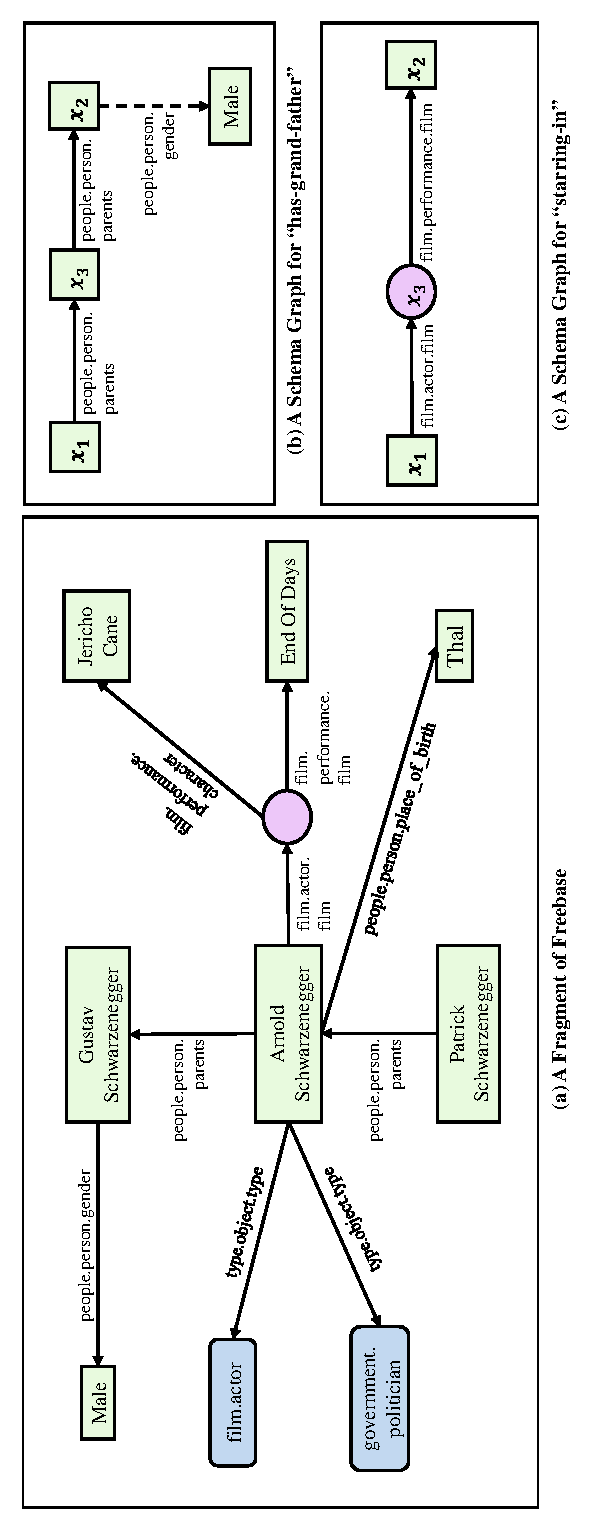
\epsfig{file=fb-schema.eps, width=0.95\columnwidth}
\centering 
\scalebox{0.7}{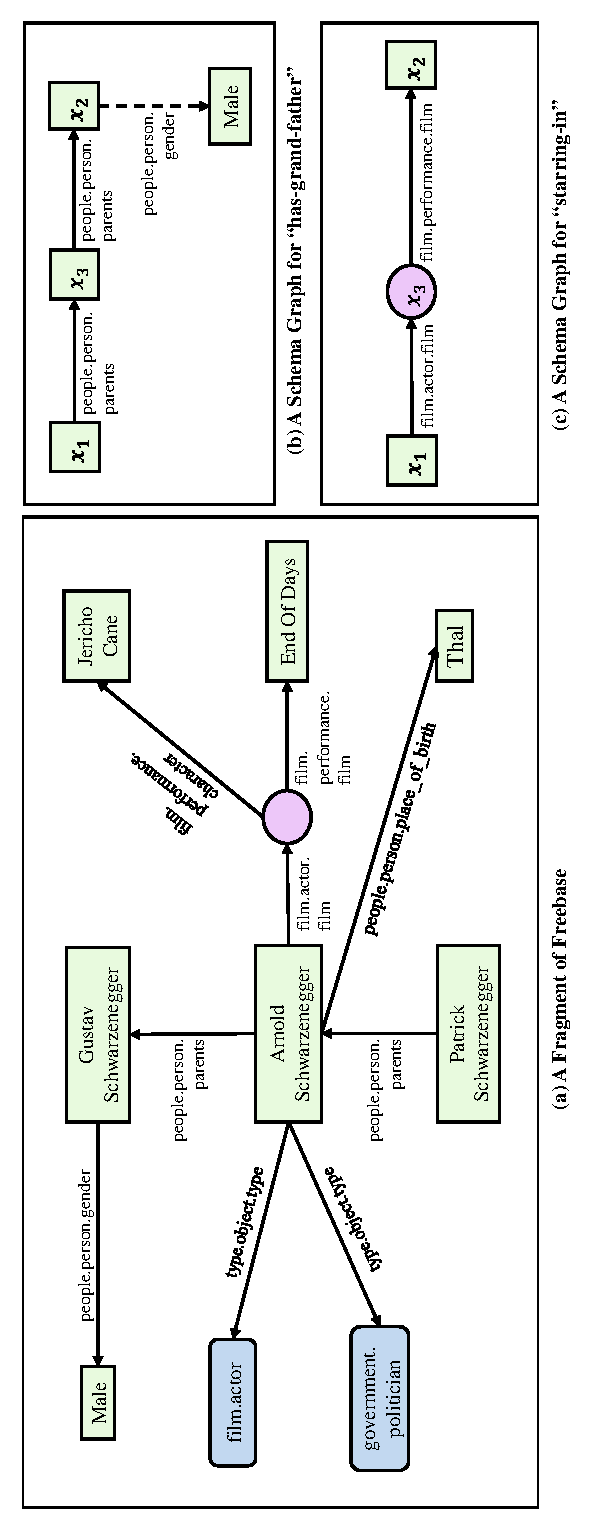
\includegraphics[angle=270]{fb-schema.eps}}
\label{fig:fb-schema}
\caption{A Fragment of Freebase and Example Schema Graphs.}
\end{figure*}

The answer to both questions lies in the ability to ``paraphrase''
a relation expressed in natural language patterns into the same relation
but represented in a knowledge graph.
For example, Freebase doesn't have grand-father-of predicate, 
or even father-of predicate, but instead has the parent-of 
and gender-of predicates, which may jointly represent the semantics of
grand-father-of (see \figref{fig:fb-schema}(b)).  


There are different ways to represent relations in a knowledge graph. 
Previous work \cite{gardnerefficient,yao2014information} on KBC proposed to represent a type
of relations by a {\em path} of predicates connecting two entities, 
along with many discriminative features on the edges and the nodes 
along the path, \KZ{For example ...}. One problem with this approach is
that the selection of such features can be random and ad hoc. 
For example, {\em anyrel} is a feature that represents any predicate 
in the knowledge graph; the difference between the numerical values 
on two different nodes can be a feature as well. A more serious
disadvantage is that such representation cannot be readily translated into
SPARQL queries. Instead additional program code must be written to support
queries, such as whether $e_1$ and $e_2$ has certain relation, or given
$e_1$ and a relation, what is $e_2$. Finally, feature-based approach
represents a relation by a bunch of weights, which are not human 
readable and are hard to explain.

Another perhaps more natural representation of a type of relation 
in a knowledge graph is a subgraph structure. This subgraph
is an abstraction of all the concrete subgraphs of the same shape
that connects each individual pair of the entities in the knowledge graph.
This subgraph connects constant entities as well as variables.
In this paper, we call such a subgraph a {\em schema graph}, or {\em schema}
in short.  A schema graph is essentially a view on the knowledge graph, 
joining several primitive relations (or predicates) together. 
For example, the grand-father-of relation can be represented by 
the Freebase schema shown in \figref{fig:fb-schema}(b), while
the starring-in relation represented in \figref{fig:fb-schema}(c).
We choose to paraphrase a natural language relation into such
a schema graph because i) it is intuitive; ii) it can be translated into
SPARQL queries straightforwardly and hence all existing RDF tools
can be used; and iii) it is human readable and allows manual fine-tuning
if necessary.

Informally, the input of paraphrasing is a list of entity pairs $(e_1, e_2)$
extracted by natural language pattern $r$, and the output is a set of 
schema graphs, ranked by their ability to represent relation $r$ in the 
knowledge graph. Obviously there are many possible schema graphs that
connect a pair of ($e_1$, $e_2$). For example, the grand-father-of relation 
maybe represented by parents + parents, or by parents + parents + gender(male). 
In general, simpler schemas tend to be more general in meaning, whereas
more complex schemas are more specific in meaning. A schema that is too general
is less expressive and less informative, while a schema that is too specific 
may not be able to cover all the entity pairs. This paper addresses this
particular trade-off.  
Previous work \cite{lao2010relational,lao2011random,zhang2012ontological} 
deals with simple schemas which are linear path between the entity pair. 

%We define the notion \textbf{simple schema}, if the schema graph cotains \textit{only}
%a path of predicates connecting entities from $e_1$ to $e_2$ in the knowledge base. 
%To this end, state-of-the-art systems have been proposed for solving this task.
%

%2. what's knowledge base try to do
%Structured knowledge base (KB) is a graph based taxonomy containing real world 
%entities,  types,  binary predicates between entities and ``IsA'' relations 
%between entities and types.
%(Machine readable, containing millions / billions of facts)

%Structured KBs such as WordNet \cite{miller1995wordnet},
%Yago \cite{suchanek2007WWW} and Freebase \cite{bollacker2008freebase} are widely used in information extraction
%and semantic learning tasks. In order to make relation schemas understood by human, we leverage types
%in the KB as the output of relation schemas.

%3. what to do is to extract schema
%The paraphrasing task is to map a natural language relation into structured
%canonical forms in KB, which is understood by both machine and human.
%
%We call the representation as \textit{relation schema} throughout this paper.
%
%\KQ{how to give a clear impression on schema}
%%\cite{bollacker2008freebase}
%%%Figure show schema on FB as the first impression (mention FB's size here)
%informal
%One can see that a relational schema is a template of many subgraphs 
%with the concrete structure in the knowledge base.
%The goal of this paper is to enable effective and efficient translation 
%process, which we call ``paraphrasing.'' 


%add. why we need to schema
%Paraphrasing is a open task, since the structured schema is an important knowledge
%used in many down-stream applications, such as question answering, text entailment
%and short text similarity querying.
%(Arguing)

%1. why we need paraphrasing

%2. what's the advantage of schema
% SPARQL query
% user intent query (check view synthesis paper)
%Paraphrasing is a fundamental task in natural language processing and understanding,
%especially in the system of question answering , 
%and knowledge base completion.
%In these tasks, the relation coming from input sentence (or question) is transformed 
%into semantic structure in the knowledge base, and the overall accuracy is largely 
%determined by the quality of the structural representation.
%
%
%There are three main advantages for our schema based model.
%First, each schema is an independent structure that represents the target relation.
%Feature weights produced by discriminative model can tell us which schemas are more
%suitable for the relation, while a single feature snippet is less expressive.
%Second, the schema is a subgraph of a semantic knowledge base. 
%Our system can easily transform a schema into a SPARQL query due to the widely used RDF model
%in semantic knowledge bases. Therefore, an end-user can query RDF to retrive instances
%or a natural language relation, even though they don't know how to write a SPARQL query.
%Third, the schema is human-readable. Interactive online QA systems can display schemas and
%allow end-users to adjust them, leading to a better user experience. 
%
%

%4. claim the gap between kb and nl on description
%Recap the semantic gap between relations and knowledge base predicates that we mentioned
%Yet some knowledge base is lack of predicates, however, the gap couldn't be removed,
%even for Freebase containing thousands of binary predicates.
%%5. simple exmple & chain example (mediator)
%%6. branching example
%%a) place_of_birth v.s. <people, was born in, place>
%%b) mediator: film.actor.film --> film.performance.film   v.s.   "starring in"
%%c) branching: female spouse v.s. "wife of"
%The predicate name ``place\_of\_birth'' in \figref{fig:fb-schema} (a) shows the difference,
%compared with relation words ``was born in''; 
%\figref{fig:fb-schema} (b) brings the gap to structural level, where the schema shows a
%complex ``parent + parent + male'' style, even ``grandfather'' relation is so common in
%the real world; Meanwhile, \figref{fig:fb-schema} (c) show that the schema must include 
%a intermediate node (used to maintain the ternary relation ``actor plays a character in a film'').
%These varieties make the paraphrase task challenging.
%
%%traditional method & limits
%%0. informally, composite relation
%%(Lei Zou) (EMNLP 2011) (AAAI 2012) (Tran 2009) (EMNLP 2015)
%For the part of feature based supervised systems, the first branch is graph-walk based 
%\cite{lao2010relational,lao2011random}, a candidate schema is drawn from the predicate path 
%between some entity pairs, and the probabilistic distribution of random walking from $e_1$ 
%to $e_2$ in KB on the schema is used as a feature to train the importance of each path.
%The second branch is logic based \cite{zhang2012ontological}, where the system uses hand 
%crafted soft rules to mine various features that leads to good relation schemas. 
%Since soft rules are fixed and independent of relations, the dimension of feature space
%is limited.
%
%Besides, unsupervised models are also used. Zou et al. \cite{zou2014natural}
%followed the idea of TF-IDF score \cite{blabla} to calculate the best schema with respect to a
%speicifc relation. While different input relations could have overlap meaning, this situation 
%causes a lower score of schemas representing the overlapping part.
%
%In addition, among all different paraphrasing solvers, the process of candidate schema 
%searching could always be a big challenge. All systems discussed above only generate
%simple schemas (predicate paths), which is also a limitation for searching more
%specific and meaningful schemas.
%
% our approach
%1. IMPORTANT data-driven
In this paper, we present a semi-supervised data-driven approach to 
solve the paraphrasing problem, with the following contributions:
\begin{itemize}
\item We give the formal definition of schemas and allow complex schemas
other than simple, linear paths to be produced, which makes paraphrasing more
accuracy and flexible (\secref{sec:problem}); 
\item Due to the prohibitive space of possible schemas, we present 
an effective local search based heuristic to generate a set of 
candidate schemas from the knowledge graph 
and score each candidate with a trained classifier (\secref{sec:candgen});
\item We propose a metric based on the \textit{Minimum Description Length}
(MDL) principle, to effectively characterize the trade-off between the simplicity
and preciseness of schemas (\secref{sec:label}); 
\item Our experiments using clean input data from Freebase 
as well as noisy inputs from PATTY
show that the proposed paraphrasing framework significantly outperforms
the state-of-the-art systems on the accuracy of knowledge base completion
task on Freebase (\secref{sec:eval}).
\end{itemize}



